\begin{figure}[t]
\centering
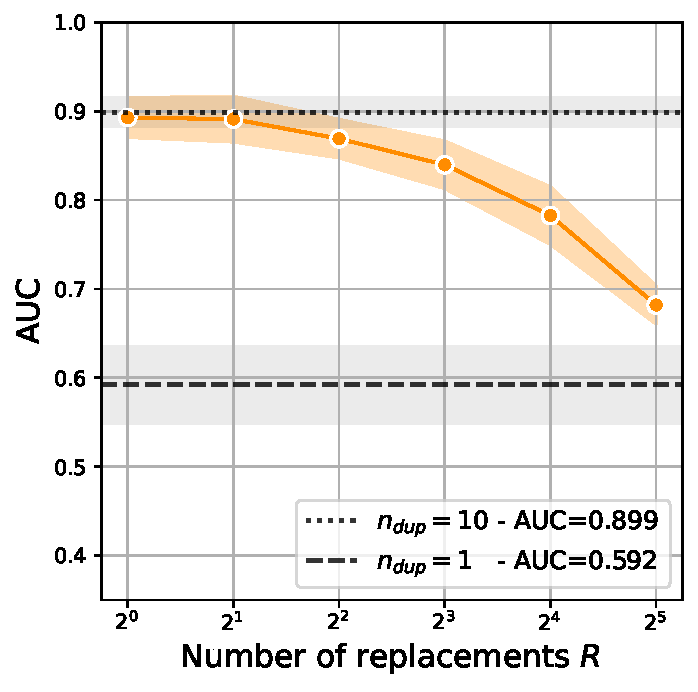
\includegraphics[width=0.8\linewidth]{figures/AUC_vs_R_main.pdf} 
    \caption{\textbf{Memorization of fuzzy trap sequences.} The \textit{Ratio} MIA performance (AUC) (mean and standard deviation) versus number of replacements $R$. For smaller values of $R$, fuzzy duplicates are memorized almost equally well than exact duplicates while for larger values of $R$, memorization remains significantly higher than for a single repetition.} 
\label{fig:auc_vs_r_main}
\end{figure} 

Large Language Models (LLMs) acquire their capabilities from the extremely large textual datasets they are trained on. These datasets mostly contain human-generated text, often also including copyright-protected content~\cite{atlantic,wired}. This raises growing concerns amongst content creators, leading some to file lawsuits against LLM developers, claiming copyright infringement for utilizing books~\cite{authorsguild,silvermanmeta}, songs~\cite{anthropic} or news articles~\cite{nytimes} for training. While the legal status of model training on copyright-protected content remains an open question in some major jurisdictions~\cite{samuelson2023generative}, new LLMs are continuously developed, often not disclosing any details on the training dataset~\cite{bommasani2023foundation,gpt4techreport,touvron2023llama2,jiang2024mixtral}. Beyond concerns on copyright, as training data fundamentally shapes the model's behaviour, data provenance becomes increasingly important to understand potential propagation of harmful content~\cite{solaiman2021process,bender2021dangers} or misinformation~\cite{zhang2023siren,barnard2023self}, and to fairly evaluate models on held-out benchmarks~\cite{magar2022data,sainz2023did,schaeffer2023pretraining}.

Recent works proposed methods to modify the original text to help content creators protect their content from being used for LLM training without consent. They propose synthetically generated \emph{copyright traps}~\cite{meeus2024copyright} or \emph{data watermarks}~\cite{wei2024proving, wang2023wasa} to be injected into the original content, potentially hidden on the web page invisible to users yet picked up by data scrapers. This enables content owners to track whether their data has been used to train newly released LLMs. They show that this injection of purposely crafted sequences enables detectability in LLMs where state-of-the-art document-level membership inference methods~\cite{meeus2023did,shi2023detecting} fail. 

However, including these traps relies on injecting long unique sequences a large number of times across the content - up to 1,000 times~\cite{meeus2024copyright}. This makes copyright traps vulnerable to accidental removal by common data preprocessing methods. Deduplication of training data has indeed been found to improve model utility and training efficiency~\cite{lee2022deduplicating,hernandez2022scaling,allamanis2019adverse,tirumala2024d4,hoffmann2022training,xue2024repeat}, which has led model developers to perform document-, and even sequence-level deduplication at scale~\cite{kudugunta2024madlad,penedo2023refinedweb}. 

\textbf{Contribution.} We propose the injection of \emph{fuzzy} copyright traps. We here measure how slight modifications across trap sequence repetitions, instead of exact duplication, impact the trap detectability, while making it increasingly hard to be removed by deduplication techniques. 

First, we introduce a framework to generate fuzzy trap sequences, each differing from a reference trap by $R$ replaced tokens. We then fine-tune the 1.3B parameter CroissantLLM~\cite{faysse2024croissantllm} on documents containing fuzzy trap sequences, and measure the trap memorization by computing the AUC of a sequence-level membership inference attack (MIA)~\cite{carlini2021extracting, kandpal2022deduplicating}. 

We find that fuzzy duplicates are memorized almost as strongly as the exact duplicates even when a significant number of tokens are replaced (see Fig.~\ref{fig:auc_vs_r_main}). For instance, the mean MIA AUC only drops from $0.90$ to $0.87$ when $R=4$ tokens are replaced in each of the 10 repetitions of a 100-token-long sequence. Compared to the baseline assumption that fuzzy duplicates do not contribute to each other's memorization (mean AUC=$0.59$), this demonstrates that LLMs possess a \emph{mosaic memory}, where the memorization of a sequence is strongly impacted by other sequences with partially overlapping fragments.

We then show how non-uniform selection of tokens to be replaced makes the method more robust to deduplication by minimizing the overlap across fuzzy trap sequences (Sec.~\ref{section:spread_replacements}). Many deduplication methods currently implemented in practice remove exact duplicates of $50$ tokens or more~\cite{lee2022deduplicating,kudugunta2024madlad,penedo2023refinedweb}. We find that, in our setup, adopting non-uniform selection reduces the number of replacements necessary to avoid removal by deduplication from $R=8$ to $R=4$, significantly increasing the memorization AUC. This shows fuzzy trap sequences to be both effective and feasible in practice.

Next, we study how different aspects of the experimental setup affect fuzzy memorization. We adapt the MIA to also leverage the fuzzy duplicates, instead of the reference trap sequence alone (Sec.~\ref{section:adapted_mia}) and study the robustness of our results to token replacement strategy and model training (Sec.~\ref{section:ablations}). We find that replacing tokens with the top predictions from a Masked Language Model boosts the MIA AUC, suggesting that semantic coherence across fuzzy duplicates improves memorization.

Second, we find that commonly used training datasets contain a significant amount of fuzzy duplicates and hence argue that our findings have implications for post-hoc studies of LLM memorization and privacy. Using the technique proposed by Lee et al.~\cite{lee2022deduplicating}, we collect all naturally occurring duplicates from The Pile~\cite{pile}, as previously used to quantify LLM memorization~\cite{carlini2022quantifying, ippolito2022preventing}. We indeed find that almost 30\% of duplicated sequences have at least one fuzzy duplicate with no more than $R=4$ token replacements. Moreover, 10\% of sequences have as many fuzzy duplicates as exact duplicates, effectively doubling the number of occurrences in the dataset. With our results demonstrating the mosaic memory effect in LLMs, we show a major confounding factor in the study of post-hoc LLM memorization relying on naturally occurring duplicates. Further, in the context of LLM privacy, our findings question the effectiveness of (exact) data deduplication as a privacy protection measure.
